\documentclass[tikz,border=4pt]{standalone}
\usepackage{ctex}
\usepackage{amsmath}
\usepackage{pgfplots}
\pgfplotsset{compat=1.18}

% p9-02b: |k|大小比较（k=2 vs k=6 vs k=12），k越大曲线离原点越远
\begin{document}
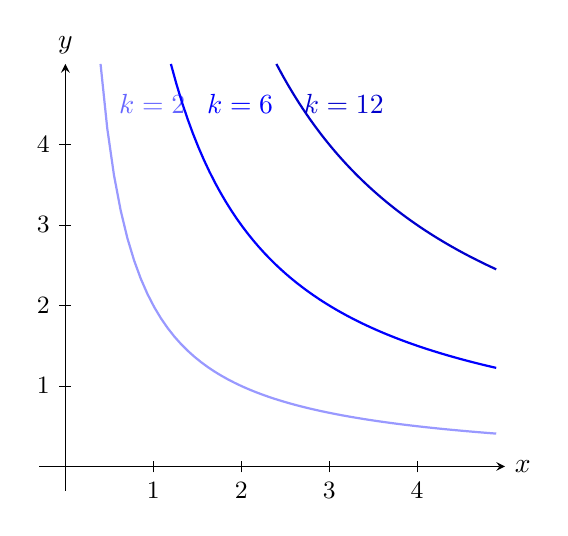
\begin{tikzpicture}
\begin{axis}[
  width=7.5cm, height=7cm,
  axis lines=center,
  xlabel={$x$}, ylabel={$y$},
  every axis x label/.style={at={(axis cs:5.0,0)}, anchor=west},
  every axis y label/.style={at={(axis cs:0,5.0)}, anchor=south},
  xmin=-0.3, xmax=5.0,
  ymin=-0.3, ymax=5.0,
  xtick={1,2,3,4},
  ytick={1,2,3,4},
  tick style={color=black},
  ticklabel style={font=\small},
  clip=true,
]
  % k=2
  \addplot[blue!40, thick, domain=0.4:4.9, samples=60] {2/x};
  \node[right, blue!60] at (axis cs:0.5, 4.5) {$k=2$};

  % k=6
  \addplot[blue, thick, domain=1.2:4.9, samples=60] {6/x};
  \node[right, blue] at (axis cs:1.5, 4.5) {$k=6$};

  % k=12
  \addplot[blue!80!black, thick, domain=2.4:4.9, samples=60] {12/x};
  \node[right, blue!80!black] at (axis cs:2.6, 4.5) {$k=12$};
\end{axis}
\end{tikzpicture}
\end{document}
